%Sie verstehen die Grundlagen eines OR-Mappers am Beispiel von Entity Framework Core
%Sie kennen die OR-Mapping-Konzepte in EF Core
%Sie kennen die Funktionalitäten der DbContext
%Sie können die CRUD-Operationen (inkl. LINQ) anwenden
%Sie können einfache Modelle erstellen und LINQ-Abfragen formulieren

\section{Entity Framework Core}
Unter .NET kommt ADO.NET als Entity Framework zum Einsatz. Man unterscheidet zwischen zwei Varianten wie die Entitätsklassen/Datenbanken erstellt werden können. Das Entity Framework muss mit NuGet installiert werden.
Es werden verschiedene Provider unterstützt: MS SQL, MySQL, PostgreSQL, SQLite, SQL Compact, in-memory.

\begin{description}
	\item[DB First] Man erstellt zuerst ein Domain Model und generiert daraus die Klassen. Man kann das Model auch von einer existierenden Datenbank ableiten und dann wieder die Klassen daraus generieren
	\item[Code First] Man erstellt die Model Klassen und lässt die Datenbank automatisch generieren.
	\item[Model First] Man erstellt zuerst das EDM (Entity Data Model) und generiert daraus die Database, sowie die Klassen
\end{description}




\subsection{OR-Mapping}
OR-Mapping ist eine Technik der Softwareentwicklung, mit der ein in einer objektorientierten Programmiersprache geschriebenes Anwendungsprogramm seine Objekte in einer relationalen Datenbank ablegen kann. EF Core verwendet für das verschiedene Provider, welche eine vielzahl von  SQL- und NoSQL-Datenbanken unterstützen.

\begin{figure}[h!]
  \center
  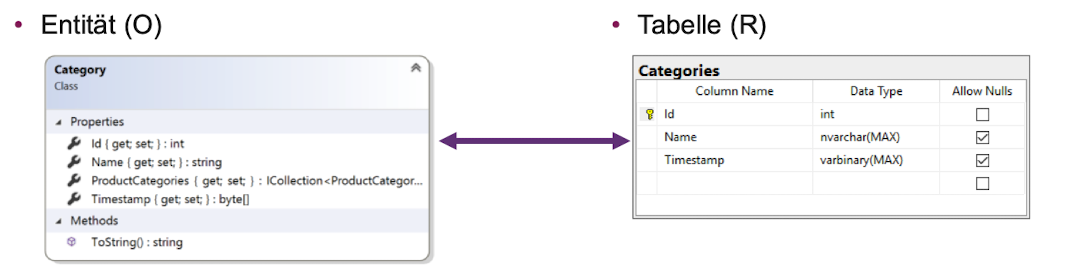
\includegraphics[width=0.75\linewidth]{OR-Mapping}
  \caption{Mapping von Objekten auf Relationen}
\end{figure}

\subsubsection{Mapping-Ansätze}
Das Mapping von Klassen auf das darunterliegende Speichermodell (Datenbank) kann auf drei verschiedene Ansätze realisiert werden. \textbf{Mapping: By Convention, By Attributes, By Fluent API}. 

\begin{minipage}{0,5\linewidth}
\begin{description}
    \item[Providers] Diverse relationale SQL Providers.
	\item[Entity] Ein Objekt mit einem Key (z.B ID). Mehrere dieser Objekte werden zu einem Entity-Set zusammengefasst.
	\item[Mapping] Mapping der Klassen auf das darunter liegende Speichermodell.
	\item[Mappingansätze] Zuordnung von Entity Type zu Storage Entity, Property zu Column, Entity Key zu Primary Key, Foreign Key zu Relationship.
	\item[Storage Entity] Relationales Modell/Graph/Collection, abhängig vom gewählten Provider. Ausprägungen: Table, View, Sotrec Procedures, etc. Inhalte: Columns, Primary KEys, Unique Key Constraints, Foreign Keys.
	\item[Association] Definiert eine Assotiation zwischen Entitäten (z.B Navigation Properties, Foreign Keys).
\end{description}

\end{minipage}
\begin{minipage}{0,5\linewidth}
	\center
  	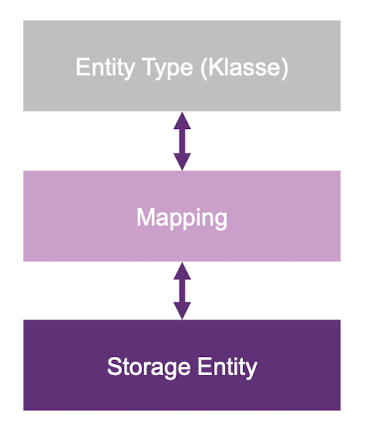
\includegraphics[width=0.5\linewidth]{or}	
\end{minipage}

\textbf{Mapping-Arten:} Das Mapping kann über das Entity-Level sowie das Attribut-Level realisiert werden.

\begin{minipage}{0,5\linewidth}
	\textbf{Entity-Level}\\
	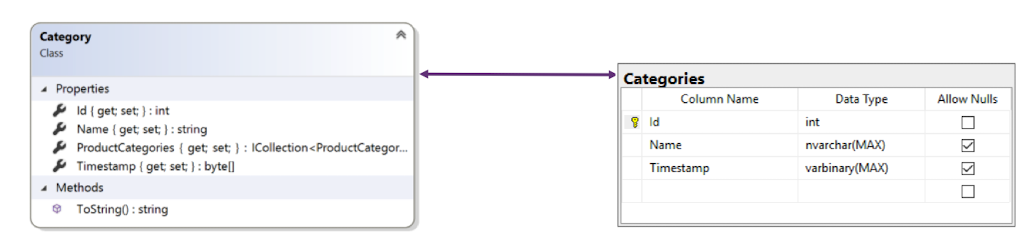
\includegraphics[width=\linewidth]{entity-level}
\end{minipage}
\begin{minipage}{0,5\linewidth}
	\textbf{Attribut-Level}\\
	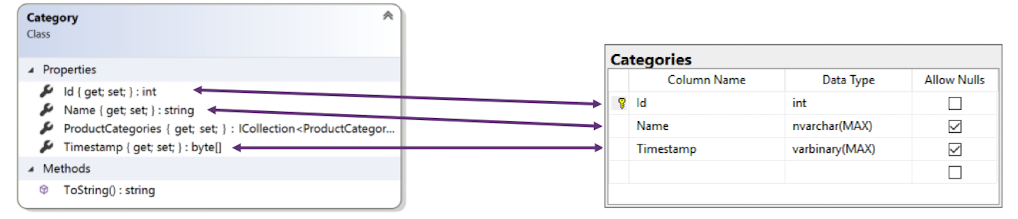
\includegraphics[width=\linewidth]{attribut-level}
\end{minipage}

\subsubsection{Model}
\begin{description}
    \item[Convention] Automatisches Mapping ohne explizite Konfiguration.
    \item[Fluent API] Extensions Method Syntax, Überschriebene Methode von ''OnModelCreating'' im DbContext \lstinline|protected override void OnModelCreating(ModelBuilder modelBuilder)|.
    \item[Data Annotations|Attributes] Deklaratives Mapping, Attribute direkt auf Model-Klassen
\end{description}

\textbf{Include/Exclude Entities}
\begin{lstlisting}
public class ShopContext : DbContext {
    // Convention - DbSet-Property im Context
    public DbSet<Category> Categories { get; set; }
    
    // Fluent API - Entry im Builder oder Ignore im Model Builder
    protected override void OnModelCreating( ModelBuilder modelBuilder) {
        modelBuilder.Entity<AuditEntry>();          
        modelBuilder.Ignore<Metadata>();
    }
}
public class Category {
    public int Id { get; set; }
    public string Name { get; set; }
    public ICollection<Product> Products { get; set; }  // Convention - Indirekt via Navigation Property
    public ICollection<Metadata> Metadata { get; set; }
}
public class Product { /* ... */ }
public class AuditEntry { /* ... */ }
[NotMapped]                               // Data Annotations
public class Metadata { /* ... */ }
\end{lstlisting}

\textbf{Include/Exclude Properties}
\begin{lstlisting}
public class ShopContext : DbContext {
    public DbSet<Category> Categories { get; set; }
    protected override void OnModelCreating(ModelBuilder modelBuilder) {
        modelBuilder.Entity<Category>()
            .Property(b => b.Name);                     
        modelBuilder.Entity<Category>()
            .Ignore(b => b.LoadedFromDatabase);  // Fluent API - Ignore im Builder
    }
}
public class Category {
    public int Id { get; set; }
    public string Name { get; set; }
    [NotMapped]                                               // Data Annotations
    public DateTime LoadedFromDatabase { get; set; }
}
\end{lstlisting}

\textbf{Keys}
\begin{lstlisting}
public class ShopContext : DbContext {
    public DbSet<Category> Categories { get; set; }
    protected override void OnModelCreating(ModelBuilder modelBuilder) {
        modelBuilder.Entity<Category>()
            .HasKey(e => e.Id)                              // Fluent API - Einzige Moeglichkeit für Composite Keys
            .IsRequired();
    }
}
public class Category {
    [Key]                                  // Data Annotations
    public int Id { get; set; }
    public string Name { get; set; }
}
public class Tanslation {
    public string Language { get; set; }
    public int CategoryId { get; set; }
}
\end{lstlisting}

\textbf{Required/Optional}
\begin{lstlisting}
public class ShopContext : DbContext {
    public DbSet<Category> Categories { get; set; }
    protected override void OnModelCreating(ModelBuilder modelBuilder) {
        modelBuilder.Entity<Category>()
            .Property(e => e.Name)
            .IsRequired();                // Fluent API
    }
}
public class Category {
    public int Id { get; set; }
    [Required]                             // Data Annotations
    public string Name { get; set; }
    public bool? IsActive { get; set; }
}
\end{lstlisting}

\textbf{Maximum Length}
Convention: Keine Restriktion / z.b. NVARCHAR(MAX), 450 Zeichen bei Keys
\begin{lstlisting}
.Property(e => e.Name).HasMaxLength(500)                 // Fluent API
[MaxLength(500)]                                         // Data Annotations
\end{lstlisting}

\textbf{Indexes} 
Convention: Werden bei Foreign Keys automatisch erstellt
\begin{lstlisting} 
modelBuilder.Entity<Category>()               // Fluent API - Non-unique Index
    .HasIndex(b => b.Name);
modelBuilder.Entity<Category>()               // Fluent API - Unique Index
    .HasIndex(b => b.Name)
    .IsUnique();
modelBuilder.Entity<Category>()               // Fluent API - Multi-column Index
    .HasIndex(b => new { b.Name, b.IsActive });
// Data Annotations - nicht unterstuetzt
\end{lstlisting}

\subsubsection{Relationale DB (SQL Server)}
\paragraph{Tabellen} Convention: Tabellenname = Klassenname (Pluralized) (z.b. dbo.Categories)
\begin{lstlisting}
// Fluent API - Name zwingend, Schema optional
modelBuilder.Entity<Category>()                         
    .ToTable("Category", schema: "dbo");
// Data Annotations - Name zwingend, Schema optional
[Table("Category", Schema = "dbo")]                     
public class Category {...}
\end{lstlisting}

\textbf{Spalten} 
Convention: Spaltenname = Property-Name
\begin{lstlisting}
// Fluent API
modelBuilder.Entity<Category>()                         
    .Property(e => e.Name)
    .HasColumnName("CategoryName", order: 1);
// Data Annotations
[Column("CategoryName", Order = 1)]                     
public string Name { get; set; }
\end{lstlisting}

\textbf{Datentypen / Default Values}
Convention: Keine Default Values
\begin{lstlisting}
// Fluent API
modelBuilder.Entity<Category>()                         
    .Property(e => e.Name)
    .HasColumnName("CategoryName")
    .HasColumnType("NVARCHAR(500)")                     // Datentyp-Name des Zielsystems
    .HasDefaultValue("---");                            // Default (Wert/Gueltige SQL Expression)
//Data Annotation - Datentyp-Name des Zielsystems, Default Values nicht unterstuetzt.
[Column("CategoryName", TypeName = "NVARCHAR(500)"] 
public string Name { get; set; }
\end{lstlisting}

\textbf{Relationship / Association – One-to-Many / Fully Defined Relationships} 
Convention: Collection Navigation Property (1-Ende), Reference Navigation Property (N-Ende), Foreign Key Property
\begin{lstlisting}
// Fluent API - HasOne/WithMany oder HasMany/WithOne
modelBuilder.Entity<Product>()
    .HasOne(p => p.Category)                            
    .WithMany(b => b.Products)
    .HasForeignKey(p => p.CategoryId)
    .HasConstraintName("FK_Product_CategoryId");
public class Product {
    public int Id { get; set; }
    public int CategoryId { get; set; }
    //Data Annotations - Auf Navigation Property wird Foreign Key Property definiert
    [ForeignKey(nameof(CategoryId))]                        
    public Category Category { get; set; }
}
public class Category {
    public int Id { get; set; }
    public ICollection<Product> Products { get; set; }
}
\end{lstlisting}

\textbf{Relationship / Association – One-to-Many / No Foreign Key Property} 
Convention: Collection Navigation Property (1-Ende), Reference Navigation Property (N-Ende)
\begin{lstlisting}
// Fluent API - .HasForeignKey weglassen
modelBuilder.Entity<Product>()
    .HasOne(p => p.Category)
    .WithMany(b => b.Products)                          
    .HasConstraintName("FK_Product_CategoryId");
public class Product {
    public int Id { get; set; }
    //Data-Annotation - Foreign Key weglassen
    public Category Category { get; set; }              
}
public class Category {
    public int Id { get; set; }
    public ICollection<Product> Products { get; set; }
}
\end{lstlisting}

\textbf{Relationship / Association – One-to-Many / Single Navigation Property} Convention: Collection Navigation Property (1-Ende)
\begin{lstlisting}
//Fluent API - .HasOne ist anders
modelBuilder.Entity<Product>()
    .HasOne<Category>()
    .WithMany(b => b.Products)
    .HasConstraintName("FK_Product_CategoryId");
public class Product {
    //Data Annotations - Foreign Key + Navigation Property weglassen
    public int Id { get; set; }                         
}
public class Category {
    public int Id { get; set; }
    public ICollection<Product> Products { get; set; }
}
\end{lstlisting}

\textbf{Relationship / Association - One-to-one / Many-to-many} One-to-one + Many-to-many

\textbf{One-to-one:} Nur Reference Navigation Property, keine Collection Navigation Property, \lstinline|.HasOne(...).WithOne(...)|

\textbf{Many-to-many:} aktuell nicht unterstützt, work-around (Assoziations-Klasse, zwei One-to-many Relationships)


\subsection{DB Context}
Der DBContext ist das Herzstück des Entity Frameworks. Er ist die Verbindung zwischen unseren Entitätsklassen und der Datenbank. Der DBContext ist verantwortlich für die Datenbankinteraktionen wie das Abfragen der Datenbank und das Laden der Daten in den Speicher als Entität. Er verfolgt auch die an der Entität vorgenommenen Änderungen und speichert die Änderungen in der Datenbank. Kombinert die Patterns: Repository, Unit of Work.

\begin{itemize}
	\item \textbf{Desing Time:} Model definierern (OR-Mapping), Konfiguration, Database Migrations.
	\item \textbf{Run-Time:} Connections verwalten, CRUD Operationen, Change Tracking, Caching, Transaction Management.
\end{itemize}

\textbf{DBContext Lifecyle}
\begin{itemize}
	\item \textbf{Sollte nicht zu lange leben:} Limitierte Anzahl Connections im Client Connection Pool, Change-Tracking wird über die Zeit ineffizient.
	\item \textbf{Sollte nicht geshared werden:} Ist nicht thread-safe, Exception kann Instanz unbrauchbar machen.
\end{itemize}

\begin{lstlisting}
using (ShopContext context = new ShopContext()) {
    /* Context / Database Operations */
}
\end{lstlisting}

\subsection{LINQ to Entities}
Das EF führt keine LINQ queries aus! Das EF Core generiert Queries und die Datenbank führt diese dann aus.
\textbf{Einfaches Beispiel}
\begin{lstlisting} 
// DbContext instanzieren, DB Verbindung oeffnen, Cache/Change Tracker initialisieren.
using (ShopContext context = new ShopContext()) {          
    Category category = context                     // Abfrage mit LINQ (direkt)
        .Categories
        .Single(c => c.Id == 1);
        
    category.Name = $"{category.Name} / Changed";     // Daten aendern / speichern 
    context.SaveChanges();
    
    var categories = context.Categories;
    foreach (Category c in categories) { Console.WriteLine(c.Name); }       // Abfrage mit LINQ (deferred)
}     // Context schliessen - Cache invalidieren / Datenbank-Verbindung zurueck in Connection Pool
\end{lstlisting}

\subsubsection{CUD Operationen (Create, Update, Delete)}
DbContext agiert nach dem Unit of Work (UoW) pattern. Objekt wird beim Laden aus der
Datenbank automatisch der UoW registriert. Änderungen werden aufgezeichnet. Beim Speichern werden alle Änderungen in einer einzigen Transaktion geschrieben.

\textbf{Insert}
\begin{lstlisting}
using (ShopContext context = new ShopContext()) {
    Category cat = new Category { Name = "Notebooks" };
    // Add to Context (3 alternatives)
    // - Use .Add(...) to apply to whole graph
    // - Use .State when only for this entity
    context.Add(cat);
    context.Categories.Add(cat);
    context.Entry(cat).State = EntityState.Added;
    // Save – SQL is executed here
    context.SaveChanges();
    // Check Primary Key
    int id = cat.Id; // Category.Id is populated
}
\end{lstlisting}

\textbf{Update}
\begin{lstlisting}
using (ShopContext context = new ShopContext()); 
Category cat = await context
	.Categories 
	.FirstAsync();
// Change 
cat.Name = "Changed";

// Save – SQL is executed here 
await context.SaveChangesAsync();
\end{lstlisting}

\textbf{Delete}
\begin{lstlisting}
using (ShopContext context = new ShopContext()) {
    Category cat = context.Categories.First(c => c.Name == "Notebooks");
    // Remove (3 alternatives)
    // - Use .Remove(...) to apply to whole graph
    // - Use .State when only for this entity
    context.Remove(cat);
    context.Categories.Remove(cat);
    context.Entry(cat).State = EntityState.Deleted;
    // Save – SQL is executed here
    context.SaveChanges();              
}
\end{lstlisting}

\subsubsection{CUD von Assozitationen}







\begin{lstlisting}
// Models
public class Blog
    {
        public int BlogId { get; set; }
        public string Url { get; set; }

        public List<Post> Posts { get; } = new();
    }

    public class Post
    {
        public Blog Blog { get; set; }
    }
}
\end{lstlisting}

\begin{lstlisting}
// DB context
public class DatabaseContext : DbContext
{
    public DbSet<Author> Authors { get; set; }
    public DbSet<Book> Books { get; set; }

	public BlogDB() : base("name=ErstesBeispiel") {
		Database.SetInitializer<BlogDB>(new DropCreateDatabaseAlways<DbContext>());
	}
}	
\end{lstlisting}

\begin{lstlisting}
// use the databse
using (var db = new BloggingContext()) {
	// Note: This sample requires the database to be created before running.
    Console.WriteLine($"Database path: {db.DbPath}.");
                
    // Create
    Console.WriteLine("Inserting a new blog");
    db.Add(new Blog { Url = "http://blogs.msdn.com/adonet" });
    db.SaveChanges();

    // Read
    Console.WriteLine("Querying for a blog");
    var blog = db.Blogs
    	.OrderBy(b => b.BlogId)
        .First();

     // Update
     Console.WriteLine("Updating the blog and adding a post");
     blog.Url = "https://devblogs.microsoft.com/dotnet";
     blog.Posts.Add(
     	new Post { Title = "Hello World", Content = "I wrote an app using EF Core!" });
     db.SaveChanges();

     // Delete
     Console.WriteLine("Delete the blog");
     db.Remove(blog);
     db.SaveChanges();
}
\end{lstlisting}

\subsection{Code First}
\subsubsection{Attribute / Data Annotations}
\begin{lstlisting}
public class Angestellter
	{
            [Key, Column("PersNr")]
            public int Id { get; set; }
            [MaxLength(20), Required]
            public string Name { get; set; }
            [Column("Tel")]
            public int? Telefonnummer { get; set; }
            [Column("Salaer", TypeName = "DECIMAL(7,2)")]
            public decimal Salaer { get; set; }
            [MaxLength(20)]
            public string Wohnort { get; set; }
            [Column(TypeName = "DATETIME")]
            public DateTime? Eintrittsdatum { get; set; }
            [Column("AbtNr")]
            public int? AbteilungId { get; set; }
            [Column(TypeName = "DECIMAL(7,2)")]
            public decimal? Bonus { get; set; }
            [Column("Chef")]
            public int? ChefId { get; set; }

            [ForeignKey(nameof(AbteilungId))]
            public virtual Abteilung Abteilung { get; set; }

        [ForeignKey(nameof(ChefId))]
        public virtual Angestellter Chef { get; set; }

        [InverseProperty(nameof(Chef))]
        public virtual ICollection<Angestellter> Unterstellte { get; set; } = new List<Angestellter>();
	} 
\end{lstlisting}

\subsection{Model Builder}
Mit dem Model Builder kann deklarativ festgelegt werden, wie das Model generiert werden soll. Das Resultat ist das selbe wie mit der Attribut Variante.

\subsection{Lazy-, Eager-Loading}
Es wird standardmässig Lazy Loading verwendet. \\
\textbf{Lazy Loading:} Daten werden erst geladen, wenn sie dereferenziert werden. z.B erst wenn effektiv auf die Membervariable (Liste aus mehreren Items) zugegriffen wird. Für das implizite Lazy Loading müssen die Methoden virtual definiert werden. \\
\textbf{Eager Loading:} Das komplette Objekt wird geladen.



\subsection{Optimistic Concurrency}
Annahme: Zwischen laden und speichern eines Datensatzes wird dieser nicht verändert. Zwei Möglichkeiten um die Änderungen zu detektieren: Timestamp / Row Version, Concurrency Tokens / Daten-Versionen. Diese werden im DBContext pro Entity definiert.

\begin{description}
  \item[Timestamp] Pro Record Timestamp / Row Version. Timestamp ist teil des Objektes
  \item[Concurrency Token] Beim laden der Daten die originalwerte wegkopieren und beim überschreiben einen Vergleich machen, ob die Daten verändert wurden.
\end{description}


\pagebreak